\chapter{AI: Algorithms}\label{AI: Algorithms}

\begin{customArrayStretch}{1.5}
\begin{longtable}{r c p{12cm}}
$V$ & 
set & 
set of vertices (nodes) of the graph \\ \hline

$E$ & 
set & 
set of edges (links) of the graph \\ \hline

$b$ & 
$\in \mathbb{R}$ & 
\textbf{branching factor} or maximum number of successors of any node \\ \hline

$d$ & 
$\in \mathbb{R}$ & 
\textbf{depth} of the \textbf{shallowest goal} node (i.e., the number of steps along the path from the root) \\ \hline

$m$ & 
$\in \mathbb{R}$ & 
maximum length of any path in the state space \\ \hline

$\varepsilon$ & $\in \mathbb{R}$ & minimum step cost (small positive constant) \\ \hline

$C$ & $\in \mathbb{R}$ & cost of the solution \\ \hline

$C^\ast$ & $\in \mathbb{R}$ & cost of the optimal solution \\ \hline

$\ell$ & $\in \mathbb{R}$ & predetermined depth limit \\ \hline

$G_n$ & node & goal node closest to $n$ \\ \hline

$M$ & $\in \mathbb{R}$ & memory bound \\ \hline

$N$ & $\in \mathbb{R}$ & total number of nodes generated \\ \hline

$k$ & $\in \mathbb{R}$ & \tableenumerate{
    \item number of restarts (for \fullref{AI: Algorithms/Random-restart hill climbing search})
    \item number of beams (for \fullref{AI: Algorithms/Local beam search})
} \\ \hline

$p$ & 
$\in \mathbb{R}$ & 
population size (for \fullref{AI: Algorithms/Genetic algorithm (GA)}) \\ \hline

$f$ & 
$\in \mathbb{R}$ & 
time to evaluate the fitness function (for \fullref{AI: Algorithms/Genetic algorithm (GA)}) \\ \hline






\hhline{===}





$g(n)$ & 
$\in \mathbb{R}$ & 
Path Cost (The \textbf{actual cost} from the \textbfit{start node} to the current node $n$) (Eg: UCS) \\ \hline

$h(n)$ & 
$\in \mathbb{R}$ & 
Heuristic Estimate (The \textbf{estimated cost} from node $n$ to the \textbfit{goal}) (Eg: GBFS, A*) \\ \hline

$f(n)$ & 
$\in \mathbb{R}$ & 
Evaluation Function (The \textbf{total estimated cost} of the \textbfit{cheapest solution} through $n$) (Eg: A*) \\ \hline

$h^\ast(n)$ & 
$\in \mathbb{R}$ & 
actual cost of getting from the root to the goal \\ \hline




\hhline{===}




$\Delta$ & 
$\in \mathbb{R}$ & 
\textbf{absolute error}: $\Delta \equiv h^\ast - h$  \\ \hline

$\epsilon$ \textbf{OR} $\Delta_r$ & 
$\in \mathbb{R}$ & 
\textbf{relative error}: $\epsilon \equiv \Delta_r \equiv (h^\ast - h)/h^\ast$ \\ \hline


$b^{\Delta_r}$ \textbf{OR} $b^\epsilon$ \textbf{OR} $b^\ast$ &
$\in \mathbb{R}$ & 
effective branching factor \\ \hline






\end{longtable}
\end{customArrayStretch}


\begin{enumerate}
    \item \textbf{heuristic function}
    \begin{enumerate}
        \item $h(n)$ = estimated cost of the cheapest path from the state at node $n$ to a goal state
        \hfill \cite{ai/book/Artificial-Intelligence-A-Modern-Approach/Russell-Norvig}

        \item Heuristic functions are the most common form in which additional knowledge of the problem is imparted to the search algorithm. 
        \hfill \cite{ai/book/Artificial-Intelligence-A-Modern-Approach/Russell-Norvig}
        
        \item if $n$ is a goal node, then $h(n)=0$
        \hfill \cite{ai/book/Artificial-Intelligence-A-Modern-Approach/Russell-Norvig}

        \item it depends only on the \textbfit{state} at that node.
        \hfill \cite{ai/book/Artificial-Intelligence-A-Modern-Approach/Russell-Norvig}

        \item the values of heuristic (eg: $h_{SLD}$) \textbf{may not} be computed from the problem description itself. Moreover, it takes a certain amount of experience to know that $h_{SLD}$ is correlated with actual road distances and is, therefore, a useful heuristic.
        \hfill \cite{ai/book/Artificial-Intelligence-A-Modern-Approach/Russell-Norvig}

        \item With a good heuristic function, however, the complexity can be reduced substantially. 
        The amount of the reduction depends on the particular problem and on the quality of the heuristic.
        \hfill \cite{ai/book/Artificial-Intelligence-A-Modern-Approach/Russell-Norvig}

        \item \textbf{admissible heuristic}: An admissible heuristic is one that \textbf{never overestimates} the cost to reach the goal. 
        Admissible heuristics are by nature optimistic because they think the cost of solving the problem is less than it actually is.
        \hfill \cite{ai/book/Artificial-Intelligence-A-Modern-Approach/Russell-Norvig}

        \item \textbf{consistency/ monotonicity}: A heuristic $h(n)$ is consistent if, for every node $n$ and every successor $n^\prime$ of $n$ generated by any action $a$, the estimated cost of reaching the goal from $n$ is no greater than the step cost of getting to $n^\prime$ plus the estimated cost of reaching the goal from $n$:
        \hfill \cite{ai/book/Artificial-Intelligence-A-Modern-Approach/Russell-Norvig}
        \\
        .\hfill $h(n) \leq c(n,\ a,\ n^\prime) + h(n^\prime)$
        \hfill \cite{ai/book/Artificial-Intelligence-A-Modern-Approach/Russell-Norvig}
        \\
        \textbf{every} consistent heuristic is also admissible
        \hfill \cite{ai/book/Artificial-Intelligence-A-Modern-Approach/Russell-Norvig}

        \item Consistency is a stricter requirement than admissibility, but one has to work quite hard to concoct heuristics that are admissible but not consistent.
        \hfill \cite{ai/book/Artificial-Intelligence-A-Modern-Approach/Russell-Norvig}

        \item if $h(n)$ is consistent, then the values of $f(n)$ along any path are non-decreasing
        \hfill \cite{ai/book/Artificial-Intelligence-A-Modern-Approach/Russell-Norvig}

        \item For almost all heuristics in practical use, the absolute error is at least proportional to the path cost $h^\ast$, so $\epsilon$ is constant or growing and the time complexity is exponential in $d$.
        \hfill \cite{ai/book/Artificial-Intelligence-A-Modern-Approach/Russell-Norvig}

        \item When the state space has many goal states - particularly \textbf{near-optimal goal} states - the search process can be led astray from the optimal path and there is an extra cost proportional to the number of goals whose cost is within a factor  of the optimal cost.
        \hfill \cite{ai/book/Artificial-Intelligence-A-Modern-Approach/Russell-Norvig}

        \item experimental measurements of b$^\ast$ on a small set of problems can provide a good guide to the heuristic’s overall usefulness. 
        A well-designed heuristic would have a value of b$^\ast$ close to $1$, allowing fairly large problems to be solved at reasonable computational cost.
        \hfill \cite{ai/book/Artificial-Intelligence-A-Modern-Approach/Russell-Norvig}

        \item \textbf{Dominating heuristic}: if for any node $n$, $h_2(n) \geq h_1(n)$, $h_2$ \textbf{dominates} $h_1$.
        Domination translates directly into efficiency: algorithm using $h_2$ will \textbf{never} expand more nodes than same algorithm using $h_1$ 
        (except possibly for some nodes with $f(n) = C^\ast$).
        \hfill \cite{ai/book/Artificial-Intelligence-A-Modern-Approach/Russell-Norvig}
        \\
        For A$^\ast$ search, every node with $f(n) < C^\ast$ will surely be expanded.
        This is the same as saying that every node with $h(n) < C^\ast - g(n)$ will surely be expanded.
        \hfill \cite{ai/book/Artificial-Intelligence-A-Modern-Approach/Russell-Norvig}

        \item One problem with generating new heuristic functions is that one often fails to get a single “clearly best” heuristic. 
        If a collection of admissible heuristics $h_1, \cdots, h_m$ is available for a problem and none of them dominates any of the others, we need not make a choice:
        \hfill \cite{ai/book/Artificial-Intelligence-A-Modern-Approach/Russell-Norvig}
        \\
        .\hfill
        $h(n) = \max\dCurlyBrac{h_1(n),\cdots,h_m(n)}$
        \hfill \cite{ai/book/Artificial-Intelligence-A-Modern-Approach/Russell-Norvig}
        \\
        This \textbf{composite heuristic} uses whichever function is most accurate on the node in question.
        Because the component heuristics are admissible, $h$ is admissible; it is also easy to prove that $h$ is consistent. 
        Furthermore, $h$ dominates all of its component heuristics.
        \hfill \cite{ai/book/Artificial-Intelligence-A-Modern-Approach/Russell-Norvig}

        \item Note that a perfect heuristic can be obtained simply by allowing h to run a full breadth-first search “on the sly”. 
        Thus, there is a tradeoff between accuracy and computation time for heuristic functions.
        \hfill \cite{ai/book/Artificial-Intelligence-A-Modern-Approach/Russell-Norvig}

        \item Admissible heuristics can also be derived from the solution cost of a \textbf{subproblem} of a given problem.
        \hfill \cite{ai/book/Artificial-Intelligence-A-Modern-Approach/Russell-Norvig}

        \item The idea behind \textbf{pattern databases} is to store these exact solution costs for every possible subproblem instance.
        We compute an admissible heuristic $h_{DB}$ for each complete state encountered during a search simply by looking up the corresponding subproblem configuration in the database. 
        The database itself is constructed by searching back from the goal and recording the cost of each new pattern encountered; the expense of this search is amortized over many subsequent problem instances.
        Each database yields an admissible heuristic, and these heuristics can be combined by taking the maximum value.
        \hfill \cite{ai/book/Artificial-Intelligence-A-Modern-Approach/Russell-Norvig}

        \item 
        \hfill \cite{ai/book/Artificial-Intelligence-A-Modern-Approach/Russell-Norvig}
    \end{enumerate}

    \item \textbf{evaluation function}:
    \begin{enumerate}
        \item The evaluation function $f$ is construed/ interpreted as a cost estimate, so the node with the lowest evaluation is expanded first.
        \hfill \cite{ai/book/Artificial-Intelligence-A-Modern-Approach/Russell-Norvig}
        
        \item The choice of $f$ determines the search strategy.
        \hfill \cite{ai/book/Artificial-Intelligence-A-Modern-Approach/Russell-Norvig}

        \item $f(n) = g(n)$ or $h(n)$ or $g(n)+h(n)$ or something else depending on the algorithm

        \item The fact that $f$-costs are \textit{non-decreasing} along any path also means that we can draw \textbf{contours} in the state space, just like the contours in a topographic map. 
        With more accurate heuristics, the bands will stretch toward the goal state and become more narrowly focused around the optimal path.
        \hfill \cite{ai/book/Artificial-Intelligence-A-Modern-Approach/Russell-Norvig}

        \item There can be exponentially many states with $f(n) < C^\ast$ even if the absolute error is bounded by a constant.
        \hfill \cite{ai/book/Artificial-Intelligence-A-Modern-Approach/Russell-Norvig}

        
    \end{enumerate}

    \item memory limitations can make a problem intractable from the point of view of computation time
    \hfill \cite{ai/book/Artificial-Intelligence-A-Modern-Approach/Russell-Norvig}

    \item The effective branching factor can vary across problem instances, but usually it is fairly constant for sufficiently hard problems.
    \hfill \cite{ai/book/Artificial-Intelligence-A-Modern-Approach/Russell-Norvig}
\end{enumerate}


\vspace{1cm}
{\centering\fontsize{25}{25}\selectfont\bfseries Classical Search Algorithms \par}
\vspace{0.5cm}

\begin{enumerate}
    \item \textbf{category of problems}: observable, deterministic, known environments where the solution is a sequence of actions
    \hfill \cite{ai/book/Artificial-Intelligence-A-Modern-Approach/Russell-Norvig}

    \item These search algorithms are designed to explore search spaces \textbf{systematically}. 
    This systematicity is achieved by keeping one or more paths in memory and by recording which alternatives have been explored at each point along the path. 
    When a goal is found, the path to that goal also constitutes a solution to the problem. 
    In many problems, however, the path to the goal is irrelevant.
    \hfill \cite{ai/book/Artificial-Intelligence-A-Modern-Approach/Russell-Norvig}
\end{enumerate}
\vspace{0.5cm}


\clearpage
{\centering\fontsize{22}{22}\selectfont\bfseries Uninformed Search/ Blind Search \par}
\vspace{0.5cm}



\section{Breadth-first search (BFS) \cite{ai/book/Artificial-Intelligence-A-Modern-Approach/Russell-Norvig}}
\label{AI: Algorithms/Breadth-first search (BFS)}


\begin{figure}[H]
    \centering
    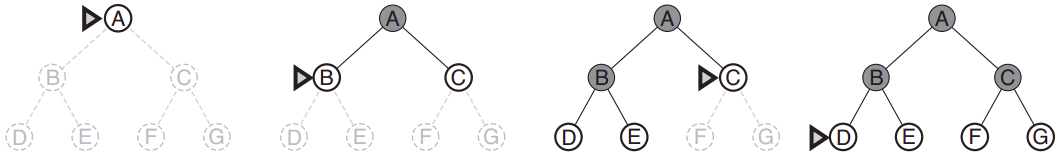
\includegraphics[
        width=\linewidth,
        height=4cm,
        keepaspectratio,
    ]{images/algorithms/Breadth-first-search-BT.png}
    \caption*{
        Breadth-first search on a simple binary tree. At each stage, the node to be expanded next is indicated by a marker.
        \cite{ai/book/Artificial-Intelligence-A-Modern-Approach/Russell-Norvig}
    }
\end{figure}


\begin{enumerate}[itemsep=0.2cm]
    \item Breadth-first search is a simple strategy in which the root node is expanded first, then all the successors of the root node are expanded next, then their successors, and so on. 
    \hfill \cite{ai/book/Artificial-Intelligence-A-Modern-Approach/Russell-Norvig}

    \item In general, all the nodes are expanded at a given depth in the search tree before any nodes at the next level are expanded.
    \hfill \cite{ai/book/Artificial-Intelligence-A-Modern-Approach/Russell-Norvig}

    \item Breadth-first search is an instance of the general graph-search algorithm in which the \textit{shallowest unexpanded node} is chosen for expansion.
    \hfill \cite{ai/book/Artificial-Intelligence-A-Modern-Approach/Russell-Norvig}

    \item new nodes (which are always deeper than their parents) go to the back of the queue, and old nodes, which are shallower than the new nodes, get expanded first. 
    \hfill \cite{ai/book/Artificial-Intelligence-A-Modern-Approach/Russell-Norvig}

    \item There is one slight tweak on the general graph-search algorithm, which is that the goal test is applied to each node when it is generated rather than when it is selected for expansion.
    \hfill \cite{ai/book/Artificial-Intelligence-A-Modern-Approach/Russell-Norvig}
    \\
    If the algorithm were to apply the goal test to nodes when selected for expansion, rather than when generated, the whole layer of nodes at depth d would be expanded before the goal was detected and the time complexity would be $\mathcal{O}(b\ ^{d+1})$.
    \hfill \cite{ai/book/Artificial-Intelligence-A-Modern-Approach/Russell-Norvig}

    \item the algorithm, following the general template for graph search, discards any new path to a state already in the frontier or explored set; it is easy to see that any such path must be at least as deep as the one already found. 
    \hfill \cite{ai/book/Artificial-Intelligence-A-Modern-Approach/Russell-Norvig}

    \item breadth-first search \textbf{always} has the \textit{shallowest path} to every node on the frontier. 
    As soon as a goal node is generated, we know it is the shallowest goal node because all shallower nodes must have been generated already and failed the goal test. 
    \hfill \cite{ai/book/Artificial-Intelligence-A-Modern-Approach/Russell-Norvig}

    \item \textbf{performance}:
    \begin{enumerate}[itemsep=0.2cm]
        \item \textbf{complete}: if the shallowest goal node is at some finite depth $d$, breadth-first search will eventually find it after generating all shallower nodes (provided the branching factor $b$ is finite). 
        \hfill \cite{ai/book/Artificial-Intelligence-A-Modern-Approach/Russell-Norvig}

        \item  the shallowest goal node is \textbf{not necessarily} the \textit{optimal} one. 
        breadth-first search is optimal if the path cost is a non-decreasing function of the depth of the node.
        The most common such scenario is that all actions have the same cost.
        the algorithm is optimal if step costs are all identical.
        \hfill \cite{ai/book/Artificial-Intelligence-A-Modern-Approach/Russell-Norvig}

        \item \textbf{Space Complexity}:
        \begin{enumerate}[itemsep=0.1cm]
            \item explored set: $\mathcal{O}(b\ ^{d-1})$
            \hfill \cite{ai/book/Artificial-Intelligence-A-Modern-Approach/Russell-Norvig}

            \item frontier: $\mathcal{O}(b\ ^{d})$
            \hfill \cite{ai/book/Artificial-Intelligence-A-Modern-Approach/Russell-Norvig}

            \item overall: $\mathcal{O}(b\ ^{d})$
            \hfill \cite{ai/book/Artificial-Intelligence-A-Modern-Approach/Russell-Norvig}
        \end{enumerate}

        \item \textbf{Time Complexity}: 
        $\mathcal{O}(b\ ^{d})$
        \hfill \cite{ai/book/Artificial-Intelligence-A-Modern-Approach/Russell-Norvig}

    \end{enumerate}

    \item \textbf{Disadvantages}:
    \begin{enumerate}[itemsep=0.1cm]
        \item the memory requirements are a bigger problem for breadth-first search than is the execution time.
        \hfill \cite{ai/book/Artificial-Intelligence-A-Modern-Approach/Russell-Norvig}

        
    \end{enumerate}

\end{enumerate}


\subsection*{Implementation}

\begin{enumerate}
    \item \textbf{frontier}: FIFO queue
\end{enumerate}


\vspace{0.5cm}


\begin{algorithm}[H]
    \caption{Breadth-first search on a graph. \cite{ai/book/Artificial-Intelligence-A-Modern-Approach/Russell-Norvig}}

    \SetKwFunction{FUNCTION}{\textsc{Breadth-First-Search}}
    \SetKwProg{Fn}{function}{ returns \normalfont{a solution, or failure}}{end}
    \Fn{\FUNCTION{problem}}{
        $node \ \gets$ a node with \textsc{State} = $problem$.\textsc{Initial-State}, \textsc{Path-Cost} = $0$ \\
        \ \\
        \If{$problem$.\textsc{Goal-Test}($node$.\textsc{State})}{
            \Return \textsc{Solution}($node$)
        }
        \ \\
        $frontier \ \gets$ a FIFO queue with node as the only element \\
        $explored \ \gets$ an empty set \\
        \ \\
        \While{}{
            \If{\textsc{Empty?}($frontier$)}{
                \Return failure
            }
            \ \\
            \Comment{chooses the shallowest node in $frontier$}
            $node \ \gets$ \textsc{Pop}($frontier$) \\ 
            add $node$.\textsc{State} to $explored$ \\
            \ \\
            \ForEach{$action$ \textbf{in} $problem$.\textsc{Actions}($node$.\textsc{State})}{
                $child \gets$ \textsc{Child-Node}($problem,\ node,\ action$) \\
                \If{$child$.\textsc{State} is \textbf{not in} $explored$ or $frontier$}{
                    \If{$problem$.\textsc{Goal-Test}($child$.\textsc{State})}{
                        \Return \textsc{Solution}($child$)
                    }
                    $frontier \gets$ \textsc{Insert}($child,\ frontier$)
                }
            }
        }
    }
\end{algorithm}


\begin{lstlisting}[
    language=Python,
    caption=Problem Solving Agent - Breadth-first search on a graph
]
from queue import Queue

def breadth_first_search(problem: Problem):
    node = Node(problem.initial_state, None, None, 0)

    if problem.goal_test(node.state):
        return solution(node)
    
    frontier = Queue()
    explored = set()

    frontier.put(node)

    while True:
        if frontier.empty():
            return None
        
        node = frontier.get()
        explored.add(node)

        for action in problem.actions(node.state):
            child = child_node(problem, node, action)
            
            if (not any([n.state == child.state for n in frontier.queue]) and 
                not any([n.state == child.state for n in explored])):
                if problem.goal_test(child.state):            
                    return solution(child)

                frontier.put(child)
\end{lstlisting}












\section{Uniform-cost search (UCS) \cite{ai/book/Artificial-Intelligence-A-Modern-Approach/Russell-Norvig}}
\label{AI: Algorithms/Uniform-cost search (UCS)}


\begin{enumerate}[itemsep=0.2cm]
    \item Instead of expanding the shallowest node (as in BFS), uniform-cost search expands the node $n$ with the \textbfit{lowest path cost} $g(n)$.
    \hfill \cite{ai/book/Artificial-Intelligence-A-Modern-Approach/Russell-Norvig}

    \item \textbf{Performance}:
    \begin{enumerate}[itemsep=0.2cm]
        \item uniform-cost search is \textbf{optimal} in general. 
        uniform-cost search expands nodes in order of their optimal path cost.
        \hfill \cite{ai/book/Artificial-Intelligence-A-Modern-Approach/Russell-Norvig}

        \item \textbf{Completeness is guaranteed} provided the cost of every step exceeds some small positive constant $\varepsilon$ and $b$ is finite
        \hfill \cite{ai/book/Artificial-Intelligence-A-Modern-Approach/Russell-Norvig}

        \item \textbf{Space Complexity}:
        \begin{enumerate}[itemsep=0.2cm]
            \item worst: $\mathcal{O}(b^{1 + \dfloor{C^\ast / \varepsilon}})$
            \hfill (can be much greater than $b^d$)
            \hfill \cite{ai/book/Artificial-Intelligence-A-Modern-Approach/Russell-Norvig}

            \item When all step costs are equal: $\mathcal{O}(b^{\ d+1})$
            \hfill \cite{ai/book/Artificial-Intelligence-A-Modern-Approach/Russell-Norvig}
        \end{enumerate}

        \item \textbf{Time Complexity}:
        \begin{enumerate}[itemsep=0.2cm]
            \item worst: $\mathcal{O}(b^{1 + \dfloor{C^\ast / \varepsilon}})$
            \hfill (can be much greater than $b^d$)
            \hfill \cite{ai/book/Artificial-Intelligence-A-Modern-Approach/Russell-Norvig}

            \item When all step costs are equal: $\mathcal{O}(b^{\ d+1})$
            \hfill \cite{ai/book/Artificial-Intelligence-A-Modern-Approach/Russell-Norvig}
        \end{enumerate}
    \end{enumerate}

    \item \textbf{Disadvantages}:
    \begin{enumerate}[itemsep=0.2cm]
        \item it will get stuck in an \textbf{infinite loop} if there is a path with an infinite sequence of \textit{zero-cost actions} - for example, a sequence of $NoOp$ actions.
        \hfill \cite{ai/book/Artificial-Intelligence-A-Modern-Approach/Russell-Norvig}

        \item  it suffers from the same difficulties with realvalued costs
        \hfill \cite{ai/book/Artificial-Intelligence-A-Modern-Approach/Russell-Norvig}
    \end{enumerate}

    \item When all step costs are the same, uniform-cost search is similar to breadth-first search, except that the latter stops as soon as it generates a goal, whereas uniform-cost search examines all the nodes at the goal’s depth to see if one has a lower cost; thus uniform-cost search does strictly more work by expanding nodes at depth $d$ unnecessarily.
    \hfill \cite{ai/book/Artificial-Intelligence-A-Modern-Approach/Russell-Norvig}
\end{enumerate}




\subsection*{Implementation}

\begin{enumerate}
    \item  This is done by storing the frontier as a \textbf{priority queue} ordered by $g(n)$. 
    \hfill \cite{ai/book/Artificial-Intelligence-A-Modern-Approach/Russell-Norvig}

    \item In addition to the ordering of the queue by path cost, there are two other significant differences from breadth-first search.
    \hfill \cite{ai/book/Artificial-Intelligence-A-Modern-Approach/Russell-Norvig}
    \begin{enumerate}
        \item  goal test is applied to a node when it is \textit{selected for expansion} rather than when it is first generated.
        The reason is that the first goal node that is \textit{generated} may be on a suboptimal path.
        \hfill \cite{ai/book/Artificial-Intelligence-A-Modern-Approach/Russell-Norvig}

        \item a test is added in case a better path is found to a node currently on the frontier.
        \hfill \cite{ai/book/Artificial-Intelligence-A-Modern-Approach/Russell-Norvig}
    \end{enumerate}

\end{enumerate}

\vspace{0.5cm}


\begin{algorithm}[H]
    \caption{\textsc{Uniform-Cost} search on a graph. \cite{ai/book/Artificial-Intelligence-A-Modern-Approach/Russell-Norvig}}

    \SetKwFunction{FUNCTION}{\textsc{Uniform-Cost-Search}}
    \SetKwProg{Fn}{function}{ returns \normalfont{a solution, or failure}}{end}
    \Fn{\FUNCTION{problem}}{
        $node \ \gets$ a node with \textsc{State} = $problem$.\textsc{Initial-State}, \textsc{Path-Cost} = $0$ \\
        $frontier \ \gets$ a \textbfit{priority queue} ordered by \textsc{Path-Cost}, with $node$ as the only element \\
        $explored \ \gets$ an empty set \\
        \ \\
        \While{}{
            \lIf{\textsc{Empty?}($frontier$)}{
                \Return failure
            }
            \Comment{chooses the lowest-cost node in $frontier$}
            $node \ \gets$ \textsc{Pop}($frontier$) \\ 
            \lIf{$problem$.\textsc{Goal-Test}($node$.\textsc{State})}{
                \Return \textsc{Solution}($node$)
            }
            add $node$.\textsc{State} to $explored$ \\
            \ \\
            \ForEach{$action$ \textbf{in} $problem$.\textsc{Actions}($node$.\textsc{State})}{
                $child \gets$ \textsc{Child-Node}($problem,\ node,\ action$) \\
                \If{\normalfont $child$.\textsc{State} is not in $explored$ or $frontier$}{
                    $frontier \gets$ \textsc{Insert}($child,\ frontier$)
                }
                \ElseIf{\normalfont $child$.\textsc{State} is in $frontier$ with higher \textsc{Path-Cost}}{
                    replace that $frontier$ node with $child$
                }
            }
        }
    }
\end{algorithm}


\begin{lstlisting}[
    language=Python,
    caption=Problem Solving Agent - Uniform cost search on a graph
]
import heapq

def uniform_cost_search(problem: Problem):
    node = Node(problem.initial_state, None, None, 0)

    if problem.goal_test(node.state):
        return solution(node)
    
    frontier = [(node.path_cost, node)]
    explored = set()

    heapq.heapify(frontier)

    while True:
        if len(frontier) == 0:
            return None
        
        path_cost, node = frontier.pop(0)

        if problem.goal_test(node.state):
            return solution(node)

        explored.add(node)
        for action in problem.actions(node.state):
            child = child_node(problem, node, action)

            if (not any([n.state == child.state for (path_cost, n) in frontier])
                and not any([n.state == child.state for n in explored])):
                frontier.append((child.path_cost, child))
                heapq.heapify(frontier)
            else:
                for idx, (path_cost, n) in enumerate(frontier):
                    if n.state == child.state and path_cost > child.path_cost:
                        frontier[idx] = (child.path_cost, child)
                        heapq.heapify(frontier)
\end{lstlisting}






\section{Depth-first search (DFS) \cite{ai/book/Artificial-Intelligence-A-Modern-Approach/Russell-Norvig}}


\begin{figure}[H]
\centering
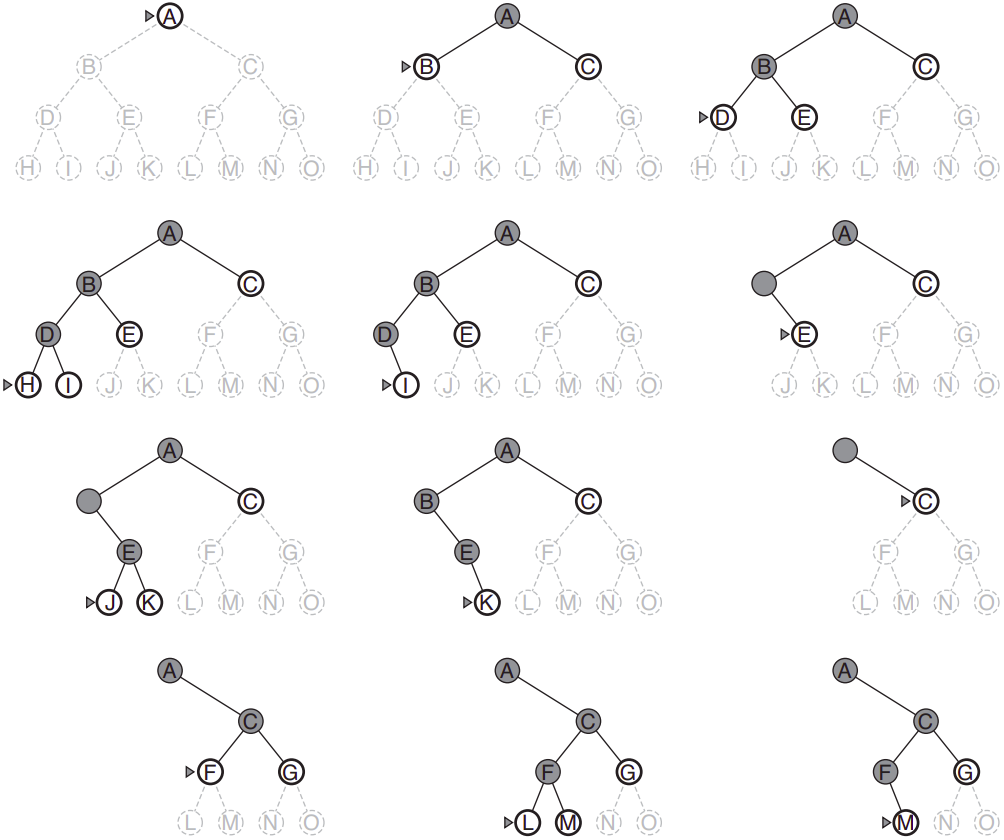
\includegraphics[
    width=\linewidth,
    height=7cm,
    keepaspectratio,
]{images/algorithms/Depth-first-search-illustration.png}
\caption*{
    Depth-first search on a binary tree. The unexplored region is shown in light gray. Explored nodes with no descendants in the frontier are removed from memory. Nodes at depth $3$ have no successors and $M$ is the only goal node. 
    \cite{ai/book/Artificial-Intelligence-A-Modern-Approach/Russell-Norvig}
}
\end{figure}


\begin{enumerate}[itemsep=0.2cm]
    \item Depth-first search always expands the \textbf{deepest node} in the current frontier of the search tree.
    \hfill \cite{ai/book/Artificial-Intelligence-A-Modern-Approach/Russell-Norvig}

    \item The search proceeds immediately to the deepest level of the search tree, where the nodes have no successors. As those nodes are expanded, they are dropped from the frontier, so then the search “backs up” to the next deepest node that still has unexplored successors.
    \hfill \cite{ai/book/Artificial-Intelligence-A-Modern-Approach/Russell-Norvig}

    \item \textbf{Performance}:
    \begin{enumerate}[itemsep=0.2cm]
        \item \textbf{graph-search version}:
        \begin{enumerate}[itemsep=0.2cm]
            \item \textbf{complete} in finite state spaces because it will eventually expand every node
            \hfill \cite{ai/book/Artificial-Intelligence-A-Modern-Approach/Russell-Norvig}

            \item \textbf{not optimal}
            \hfill \cite{ai/book/Artificial-Intelligence-A-Modern-Approach/Russell-Norvig}

            \item \textbf{time complexity}: $\mathcal{O}(b^d)$
            \hfill \cite{ai/book/Artificial-Intelligence-A-Modern-Approach/Russell-Norvig}

            \item \textbf{space complexity}: $\mathcal{O}(b^d)$
            \hfill \cite{ai/book/Artificial-Intelligence-A-Modern-Approach/Russell-Norvig}
        \end{enumerate}

        \item \textbf{tree-search version}:
        \begin{enumerate}[itemsep=0.2cm]
            \item \textbf{not complete}, as it can fall in \textit{infinite loop}
            \hfill \cite{ai/book/Artificial-Intelligence-A-Modern-Approach/Russell-Norvig}

            \item \textbf{not optimal}
            \hfill \cite{ai/book/Artificial-Intelligence-A-Modern-Approach/Russell-Norvig}

            \item \textbf{time complexity}: $\mathcal{O}(b^m)$
            \hfill \cite{ai/book/Artificial-Intelligence-A-Modern-Approach/Russell-Norvig}

            \item \textbf{space complexity}: $\mathcal{O}(b\ m)$
            \hfill \cite{ai/book/Artificial-Intelligence-A-Modern-Approach/Russell-Norvig}
        \end{enumerate}
    \end{enumerate}
\end{enumerate}


\subsection{Implementation}

\begin{enumerate}[itemsep=0.2cm]
    \item The depth-first search algorithm is an instance of the graph-search algorithm that uses a LIFO queue.
    \hfill \cite{ai/book/Artificial-Intelligence-A-Modern-Approach/Russell-Norvig}

    \item  it is common to implement depth-first search with a recursive function that calls itself  on each of its children in turn. 
    \hfill \cite{ai/book/Artificial-Intelligence-A-Modern-Approach/Russell-Norvig}
\end{enumerate}

\begin{lstlisting}[
    language=Python,
    caption=Problem Solving Agent - Depth first search on a graph
]
from queue import LifoQueue

def depth_first_search(problem: Problem):
    node = Node(problem.initial_state, None, None, 0)

    if problem.goal_test(node.state):
        return solution(node)
    
    frontier = LifoQueue()
    explored = set()

    frontier.put(node)

    while True:
        if frontier.empty():
            return None
        
        node = frontier.get()
        explored.add(node)

        for action in problem.actions(node.state):
            child = child_node(problem, node, action)

            if (not any([n.state == child.state for n in frontier.queue]) and 
                not any([n.state == child.state for n in explored])):
                if problem.goal_test(child.state):
                    return solution(child)

                frontier.put(child)
\end{lstlisting}















\section{Backtracking Search \cite{ai/book/Artificial-Intelligence-A-Modern-Approach/Russell-Norvig}}
\label{AI: Algorithms/Backtracking Search}


\begin{enumerate}
    \item A variant of depth-first search that uses still less memory.
    \hfill \cite{ai/book/Artificial-Intelligence-A-Modern-Approach/Russell-Norvig}

    \item \textbf{only one successor} is generated at a time rather than all successors; each partially expanded node remembers which successor to generate next.
    \hfill \cite{ai/book/Artificial-Intelligence-A-Modern-Approach/Russell-Norvig}

    \item \textbf{Performance}:
    \begin{enumerate}
        \item \textbf{Space Complexity}: $\mathcal{O}(m)$
        \hfill \cite{ai/book/Artificial-Intelligence-A-Modern-Approach/Russell-Norvig}
    \end{enumerate}

    \item \textbf{Advantages}:
    \begin{enumerate}
        \item  Backtracking search facilitates memory-saving (and time-saving) trick: the idea of generating a successor by \textbf{modifying} the current state description directly rather than copying it first.
        For this to work, we must be able to \textbf{undo} each modification when we go back to generate the next successor.
        \hfill \cite{ai/book/Artificial-Intelligence-A-Modern-Approach/Russell-Norvig}

        \item For problems with large state descriptions, such as robotic assembly, these techniques are critical to success.
        \hfill \cite{ai/book/Artificial-Intelligence-A-Modern-Approach/Russell-Norvig}
    \end{enumerate}
\end{enumerate}



\begin{lstlisting}[
    language=Python,
    caption=Problem Solving Agent - Backtracking using recursion \cite{common/online/chatgpt}
]
def backtrack(node: Node, explored: set):
    if problem.goal_test(node.state):
        return solution(node)

    explored.add(node)

    for action in problem.actions(node.state):
        child = child_node(problem, node, action)
        if not any([child.state == n.state for n in explored]):
            result = backtrack(child, explored)
            if result is not None:
                return result

    # Optional: allow revisiting for other paths (depends on problem)
    explored.remove(node)
    return None

def backtracking_search(problem: Problem):
    root = Node(problem.initial_state, None, None, 0)
    return backtrack(root, set())
\end{lstlisting}















\section{Depth-limited search \cite{ai/book/Artificial-Intelligence-A-Modern-Approach/Russell-Norvig}}

\begin{enumerate}[itemsep=0.2cm]
    \item The embarrassing failure of depth-first search in infinite state spaces can be alleviated by supplying depth-first search with a predetermined depth limit $\ell$. That is, nodes at depth  $\ell$ are treated as if they have no successors. 
    \hfill \cite{ai/book/Artificial-Intelligence-A-Modern-Approach/Russell-Norvig}

    \item \textbf{Performance}:
    \begin{enumerate}
        \item \textbf{Completeness}: NO \textbf{if} $\ell < d$ \textbf{else} YES
        \hfill \cite{ai/book/Artificial-Intelligence-A-Modern-Approach/Russell-Norvig}

        \item \textbf{Optimal}: NO \textbf{if} $\ell > d$ \textbf{else} YES
        \hfill \cite{ai/book/Artificial-Intelligence-A-Modern-Approach/Russell-Norvig}

        \item \textbf{time complexity}: $\mathcal{O}(b^\ell)$
        \hfill \cite{ai/book/Artificial-Intelligence-A-Modern-Approach/Russell-Norvig}

        \item \textbf{space complexity}: $\mathcal{O}(b\ell)$
        \hfill \cite{ai/book/Artificial-Intelligence-A-Modern-Approach/Russell-Norvig}
    \end{enumerate}

    \item Depth-first search can be viewed as a special case of depth-limited search with $\ell = \infty$.
    \hfill \cite{ai/book/Artificial-Intelligence-A-Modern-Approach/Russell-Norvig}

    \item diameter of the state space can be a better limit for efficiency
    \hfill \cite{ai/book/Artificial-Intelligence-A-Modern-Approach/Russell-Norvig}

    
\end{enumerate}


\vspace{0.5cm}

\begin{algorithm}[H]
    \caption{A recursive implementation of depth-limited tree search. \cite{ai/book/Artificial-Intelligence-A-Modern-Approach/Russell-Norvig}}


    \SetKwFunction{FUNCTION}{\textsc{Depth-Limited-Search}}
    \SetKwProg{Fn}{function}{ returns \normalfont{a solution, or failure/cutoff}}{end}
    \Fn{\FUNCTION{problem, limit}}{
        \Return \textsc{Recursive-DLS}( \\
            \hspace{0.5cm}  \textsc{Make-Node}($problem$.\textsc{Initial-State}), \\
            \hspace{0.5cm}  $problem$, \\
            \hspace{0.5cm}  $limit$, \\
        )
    }
    
    \ \\
    
    \SetKwFunction{FUNCTION}{\textsc{Recursive-DLS}}
    \SetKwProg{Fn}{function}{ returns \normalfont{a solution, or failure/cutoff}}{end}
    \Fn{\FUNCTION{node, problem, limit}}{
        \If{\normalfont $problem$.\textsc{Goal-Test}($node$.\textsc{State})}{
            \Return \textsc{Solution}($node$) 
        }
        \ElseIf{limit = 0}{
            \Return $cutoff$
        }
        \Else{
            $cutoff\_occurred? \ \gets$ false\\
            \ \\
            \ForEach{\normalfont $action$ \textbf{in} $problem$.\textsc{Actions}($node$.\textsc{State})}{
                $child \gets$ \textsc{Child-Node}($problem,\ node,\ action$)\\
                $result \gets$ \textsc{Recursive-DLS}($child,\ problem,\ limit-1$)\\
                \If{result = cutoff}{
                    $cutoff\_occurred? \ \gets$ true
                }
                \ElseIf{result $\neq$ failure}{
                    \Return $result$
                }
            }
            \ \\
            \If{$cutoff\_occurred?$}{
                \Return $cutoff$
            }
            \Else{
                \Return $failure$
            }
        }
    }
\end{algorithm}


\begin{lstlisting}[
    language=Python,
    caption=Problem Solving Agent - Depth limited search (recursive)
]
CUTOFF = "CUT-OFF"

def depth_limited_search(problem: Problem, limit: int):
    return recursive_dls(
        Node(problem.initial_state, None, None, 0),
        problem,
        limit,
    )

def recursive_dls(node: Node, problem: Problem, limit: int):
    if problem.goal_test(node.state):
        return solution(node)
    
    elif limit == 0:
        return CUTOFF
    
    else:
        cutoff_occurred = False
        for action in problem.actions(node.state):
            child = child_node(problem, node, action)
            result = recursive_dls(child, problem, limit-1)
            if result == CUTOFF:
                cutoff_occurred = True
            elif result is not None:
                return result
        if cutoff_occurred:
            return CUTOFF
        else:
            return
\end{lstlisting}


\vspace{0.5cm}

\begin{enumerate}[itemsep=0.2cm]
    \item $failure$ value indicates no solution
    \hfill \cite{ai/book/Artificial-Intelligence-A-Modern-Approach/Russell-Norvig}

    \item $cutoff$ value indicates no solution within the depth limit
    \hfill \cite{ai/book/Artificial-Intelligence-A-Modern-Approach/Russell-Norvig}
\end{enumerate}








\section{Iterative Deepening Search (IDS) \cite{ai/book/Artificial-Intelligence-A-Modern-Approach/Russell-Norvig}}
\label{AI: Algorithms/Iterative Deepening Search (IDS)}


\begin{figure}[h!]
    \centering
    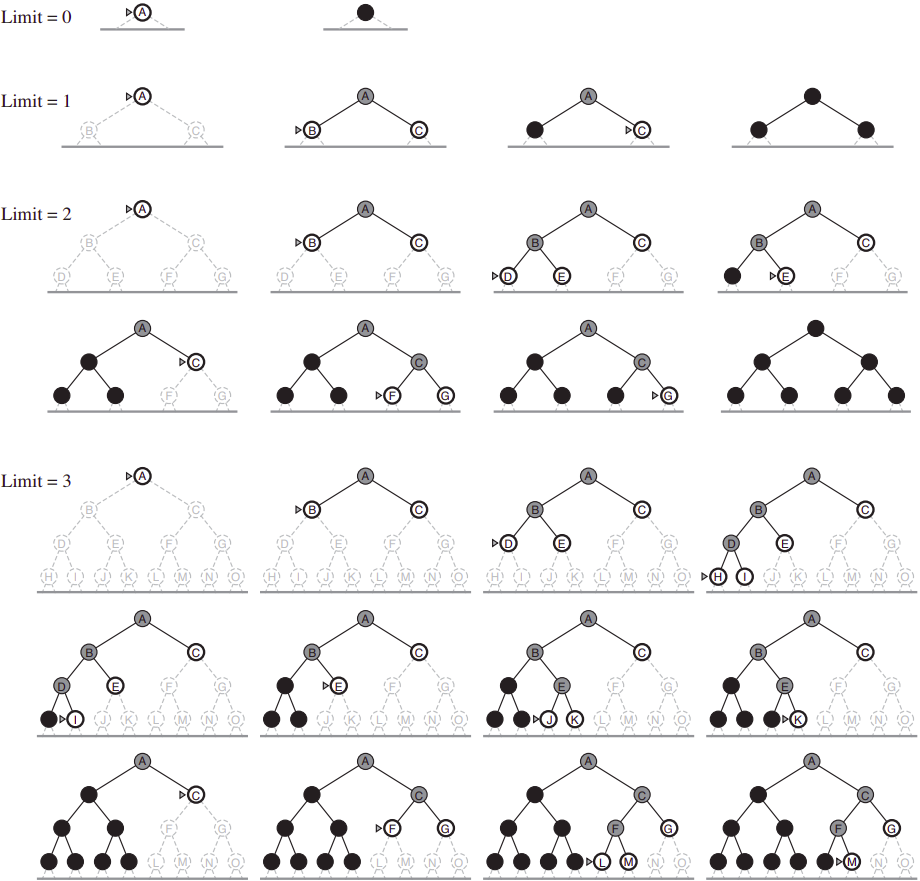
\includegraphics[
        width=\linewidth,
        height=14cm,
        keepaspectratio,
    ]{images/algorithms/iterative-deepening-search-BT.png}
    \caption*{Four iterations of iterative deepening search on a binary tree \cite{ai/book/Artificial-Intelligence-A-Modern-Approach/Russell-Norvig}}
\end{figure}


\begin{enumerate}
    \item \textbf{Iterative deepening search} (or \textbf{iterative deepening depth-first search}) is a general strategy, often used in combination with depth-first tree search, that finds the best depth limit.
    \hfill \cite{ai/book/Artificial-Intelligence-A-Modern-Approach/Russell-Norvig}

    \item It gradually increases the depth limit $\ell \in \dCurlyBrac{0,1,2,\cdots,\infty}$ till a goal is found, which occurs when $\ell = d$ ($d$ is unknown in reality)
    \hfill \cite{ai/book/Artificial-Intelligence-A-Modern-Approach/Russell-Norvig}

    \item Iterative deepening combines the benefits of depth-first and breadth-first search.
    \hfill \cite{ai/book/Artificial-Intelligence-A-Modern-Approach/Russell-Norvig}
    \begin{enumerate}
        \item Like depth-first search, its memory requirements are modest: $\mathcal{O}(b d)$ to be precise. 
        \hfill \cite{ai/book/Artificial-Intelligence-A-Modern-Approach/Russell-Norvig}

        \item Like breadth-first search, it is complete when the branching factor is finite and optimal when the path cost is a non-decreasing function of the depth of the node.
        \hfill \cite{ai/book/Artificial-Intelligence-A-Modern-Approach/Russell-Norvig}
    \end{enumerate}

    \item total number of nodes generated in the worst case is
    \\
    $N(\text{IDS})=(d)b + (d - 1)b^2 + \cdots + (1)b^d$
    \hfill \cite{ai/book/Artificial-Intelligence-A-Modern-Approach/Russell-Norvig}

    \item you can use a hybrid approach that runs breadth-first search until almost all the available memory is consumed, and then runs iterative deepening from all the nodes in the frontier.
    \hfill \cite{ai/book/Artificial-Intelligence-A-Modern-Approach/Russell-Norvig}

    \item iterative deepening is the \textit{preferred uninformed search} method when the search space is large and the depth of the solution is not known.
    \hfill \cite{ai/book/Artificial-Intelligence-A-Modern-Approach/Russell-Norvig}

    \item \textbf{Performance}:
    \begin{enumerate}
        \item \textbf{completeness}: YES \textbf{if} $b$ is finite \textbf{else} NO
        \hfill \cite{ai/book/Artificial-Intelligence-A-Modern-Approach/Russell-Norvig}

        \item \textbf{optimal}: YES \textbf{if} path cost is a non-deceasing function of depth of the node \textbf{else} NO
        \hfill \cite{ai/book/Artificial-Intelligence-A-Modern-Approach/Russell-Norvig}
        
        \item \textbf{space complexity}: $\mathcal{O}(b d)$
        \hfill \cite{ai/book/Artificial-Intelligence-A-Modern-Approach/Russell-Norvig}

        \item \textbf{time complexity}: $\mathcal{O}(b^d)$
        \hfill \cite{ai/book/Artificial-Intelligence-A-Modern-Approach/Russell-Norvig}
    \end{enumerate}
\end{enumerate}

\vspace{0.5cm}

\begin{algorithm}[H]
    \caption{The iterative deepening search algorithm, which repeatedly applies depth-limited search with increasing limits. It terminates when a solution is found or if the depth-limited search returns failure, meaning that no solution exists. \cite{ai/book/Artificial-Intelligence-A-Modern-Approach/Russell-Norvig}}

    \SetKwFunction{FUNCTION}{\textsc{Iterative-Deepening-Search}}
    \SetKwProg{Fn}{function}{ returns \normalfont{a solution, or failure}}{end}
    \Fn{\FUNCTION{problem}}{
        \For{\normalfont $depth = 0$ \textbf{to} $\infty$}{
            $result \gets$ \textsc{Depth-Limited-Search}($problem,\ depth$)\\
            \lIf{$result \neq cutoff$}{
                \Return $result$
            }
        }
    }
\end{algorithm}


\begin{lstlisting}[
    language=Python,
    caption=Problem Solving Agent - Iterative Deepening Search 
]
def iterative_deepening_search(problem: Problem, limit=1000000):
    for i in range(limit):
        result = depth_limited_search(problem, i)
        if result != CUTOFF:
            return result
\end{lstlisting}







\section{Iterative Lengthening Search (ILS) \cite{ai/book/Artificial-Intelligence-A-Modern-Approach/Russell-Norvig}}
\label{AI: Algorithms/Iterative Lengthening Search (ILS)}


\begin{enumerate}
    \item an iterative analog to uniform-cost search, inheriting the Iterative deepening search algorithm’s optimality guarantees while avoiding its memory requirements. The idea is to use increasing path-cost limits instead of increasing depth limits.
    \hfill \cite{ai/book/Artificial-Intelligence-A-Modern-Approach/Russell-Norvig}

    \item \textbf{Disadvantage}: It turns out that iterative lengthening incurs substantial overhead compared to uniform-cost search.
    \hfill \cite{ai/book/Artificial-Intelligence-A-Modern-Approach/Russell-Norvig}
\end{enumerate}


\vspace{0.5cm}


\begin{lstlisting}[
    language=Python,
    caption=Problem Solving Agent - Iterative Lengthening Search \cite{common/online/chatgpt}
]
def iterative_lengthening_search(problem: Problem):
    cost_limit = 0

    while True:
        result, new_cost_limit = uniform_cost_search_with_cost_limit(
            problem,
            cost_limit,
        )

        if result is not None:
            return result

        if new_cost_limit == float('inf'):
            return None

        cost_limit = new_cost_limit


def uniform_cost_search_with_cost_limit(problem: Problem, cost_limit: int):
    node = Node(problem.initial_state, None, None, 0)

    if problem.goal_test(node.state):
        return solution(node), cost_limit

    frontier = [(node.path_cost, node)]
    explored = set()
    heapq.heapify(frontier)
    next_cost_limit = float('inf')

    while frontier:
        path_cost, node = heapq.heappop(frontier)

        if path_cost > cost_limit:
            next_cost_limit = min(next_cost_limit, path_cost)
            continue

        if problem.goal_test(node.state):
            return solution(node), cost_limit

        explored.add(node)

        for action in problem.actions(node.state):
            child = child_node(problem, node, action)

            if (not any(child.state == n.state for n in explored) and
                not any(n.state == child.state for _, n in frontier)):
                heapq.heappush(frontier, (child.path_cost, child))

    return None, next_cost_limit
\end{lstlisting}







\section{Bidirectional search \cite{ai/book/Artificial-Intelligence-A-Modern-Approach/Russell-Norvig}}
\label{AI: Algorithms/Bidirectional search}

\begin{figure}[h!]
    \centering
    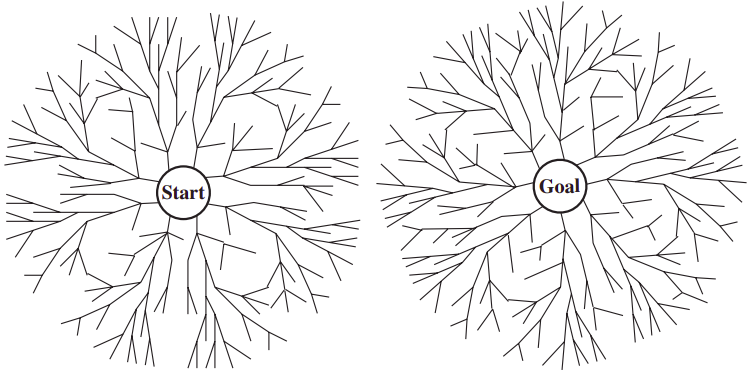
\includegraphics[
        width=\linewidth,
        height=4cm,
        keepaspectratio,
    ]{images/algorithms/bidirectional-search-illustration.png}
    \caption*{A schematic view of a bidirectional search that is about to succeed when a branch from the start node meets a branch from the goal node. \cite{ai/book/Artificial-Intelligence-A-Modern-Approach/Russell-Norvig}}
\end{figure}


\begin{enumerate}[itemsep=0.2cm]
    \item The idea behind bidirectional search is to run two simultaneous searches - one forward from the initial state and the other backward from the goal - hoping that the two searches meet in the middle
    \hfill \cite{ai/book/Artificial-Intelligence-A-Modern-Approach/Russell-Norvig}

    \item The motivation is that $b^{d/2} + b^{d/2}$ is much less than $b^d$
    \hfill \cite{ai/book/Artificial-Intelligence-A-Modern-Approach/Russell-Norvig}

    \item Bidirectional search is implemented by replacing the goal test with a check to see whether the frontiers of the two searches intersect; if they do, a solution has been found.
    \hfill \cite{ai/book/Artificial-Intelligence-A-Modern-Approach/Russell-Norvig}

    \item The check can be done when each node is generated or selected for expansion and, with a hash table, will take constant time.
    \hfill \cite{ai/book/Artificial-Intelligence-A-Modern-Approach/Russell-Norvig}

    \item \textbf{predecessors} of a state $x$ be all those states that have $x$ as a successor. Bidirectional search requires a method for computing predecessors. When all the actions in the state space are reversible, the predecessors of $x$ are just its successors. 
    \hfill \cite{ai/book/Artificial-Intelligence-A-Modern-Approach/Russell-Norvig}

    \item \textbf{Performance}:
    \begin{enumerate}
        \item \textbf{optimality}: 
        \begin{enumerate}
            \item YES \textbf{if} additional search is used to make sure the path isn’t another short-cut across the gap \textbf{else} NO
            \hfill \cite{ai/book/Artificial-Intelligence-A-Modern-Approach/Russell-Norvig}

            \item YES \textbf{if}  step costs are all identical \textbfit{and} both directions use breadth-first search \textbf{else} NO
            \hfill \cite{ai/book/Artificial-Intelligence-A-Modern-Approach/Russell-Norvig}
        \end{enumerate}

        \item \textbf{completeness}: YES \textbf{if} $b$ is finite \textbfit{and} both directions use breadth-first search \textbf{else} NO
        \hfill \cite{ai/book/Artificial-Intelligence-A-Modern-Approach/Russell-Norvig}

        \item \textbf{space complexity}:
        \begin{enumerate}
            \item using breadth-first searches in both directions: $\mathcal{O}(b^{d/2})$
            \hfill \cite{ai/book/Artificial-Intelligence-A-Modern-Approach/Russell-Norvig}
        \end{enumerate}

        \item \textbf{time complexity}:
        \begin{enumerate}
            \item using breadth-first searches in both directions: $\mathcal{O}(b^{d/2})$
            \hfill \cite{ai/book/Artificial-Intelligence-A-Modern-Approach/Russell-Norvig}
        \end{enumerate}
    \end{enumerate}
\end{enumerate}

























\clearpage
{\centering\fontsize{22}{22}\selectfont\bfseries Informed Search/ Heuristic Search \par}
\vspace{0.5cm}

\section{Best-first search (BestFS) \cite{ai/book/Artificial-Intelligence-A-Modern-Approach/Russell-Norvig}}
\label{AI: Algorithms/Best-first search (BestFS)}


\begin{enumerate}
    \item Best-first search is an instance of the general \textsc{Tree-Search} or \textsc{Graph-Search} algorithm in which a node is selected for expansion based on an \textbf{evaluation function}, $f(n)$. $f(n)$ can be any function that returns a value for a given node.
    \hfill \cite{ai/book/Artificial-Intelligence-A-Modern-Approach/Russell-Norvig}

    \item The implementation of best-first graph search is identical to that for uniform-cost search, except for the use of $f$ instead of $g$ to order the priority queue.
    \hfill \cite{ai/book/Artificial-Intelligence-A-Modern-Approach/Russell-Norvig}

    \item Most best-first algorithms include $h$ as a component of $f$
    \hfill \cite{ai/book/Artificial-Intelligence-A-Modern-Approach/Russell-Norvig}
\end{enumerate}


\begin{lstlisting}[
    language=Python,
    caption=Problem Solving Agent - (General) Best-first search (BestFS) on a graph
]
def best_first_search(problem: Problem, f):
    node = Node(problem.initial_state, None, None, 0)

    if problem.goal_test(node.state):
        return solution(node)

    frontier = [(f(node), node)]
    heapq.heapify(frontier)
    explored = set()

    while frontier:
        _, node = heapq.heappop(frontier)

        if problem.goal_test(node.state):
            return solution(node)

        explored.add(node)

        for action in problem.actions(node.state):
            child = child_node(problem, node, action)
            if (all(n.state != child.state for n in explored) 
                and all(n.state != child.state for _, n in frontier)):
                heapq.heappush(frontier, (f(child), child))
            else:
                # Optional: Replace in frontier if better
                for i, (old_f, old_node) in enumerate(frontier):
                    if old_node.state == child.state and f(child) < old_f:
                        frontier[i] = (f(child), child)
                        heapq.heapify(frontier)
                        break

    return None
\end{lstlisting}





\section{Greedy best-first search (GBFS) \cite{ai/book/Artificial-Intelligence-A-Modern-Approach/Russell-Norvig}}
\label{AI: Algorithms/Greedy best-first search (GBFS)}

.\hfill
$f(n) = h(n)$
\hfill \cite{ai/book/Artificial-Intelligence-A-Modern-Approach/Russell-Norvig}

\ \\

\begin{enumerate}
    \item Greedy best-first search tries to expand the node that is \textbf{closest} to the goal, on the grounds that this is likely to lead to a solution quickly.
    \hfill \cite{ai/book/Artificial-Intelligence-A-Modern-Approach/Russell-Norvig}

    \item at each step it tries to get as close to the goal as it can
    \hfill \cite{ai/book/Artificial-Intelligence-A-Modern-Approach/Russell-Norvig}

    \item \textbf{Performance}:
    \begin{enumerate}
        \item \textbf{Completeness}: YES \textbf{if} graph version is used \textbf{and} states are finite \textbf{else} NO
        \hfill \cite{ai/book/Artificial-Intelligence-A-Modern-Approach/Russell-Norvig}

        \item \textbf{time complexity}
        \begin{enumerate}
            \item worst case: $\mathcal{O}(b^m)$
            \hfill \cite{ai/book/Artificial-Intelligence-A-Modern-Approach/Russell-Norvig}
        \end{enumerate}

        \item \textbf{space complexity}
        \begin{enumerate}
            \item worst case: $\mathcal{O}(b^m)$
            \hfill \cite{ai/book/Artificial-Intelligence-A-Modern-Approach/Russell-Norvig}
        \end{enumerate}
    \end{enumerate}
\end{enumerate}




\begin{lstlisting}[
    language=Python,
    caption=Problem Solving Agent - Greedy Best-first search (GBFS) on a graph
]
import heapq

def greedy_best_first_search(problem: Problem):
    node = Node(problem.initial_state, None, None, 0)

    if problem.goal_test(node.state):
        return solution(node)

    # Priority queue ordered by heuristic cost
    frontier = [(problem.heuristic(node.state), node)]
    heapq.heapify(frontier)

    explored = set()

    while len(frontier) > 0:
        _, node = heapq.heappop(frontier)

        if problem.goal_test(node.state):
            return solution(node)

        explored.add(node)

        for action in problem.actions(node.state):
            child = child_node(problem, node, action)
            h_cost = problem.heuristic(child.state)

            # Add child only if it's not in frontier or explored
            in_frontier = any(n.state == child.state for _, n in frontier)
            in_explored = any(n.state == child.state for n in explored)

            if not in_frontier and not in_explored:
                heapq.heappush(frontier, (h_cost, child))
            else:
                # Optional: If it's in the frontier but has a
                # better heuristic, replace it
                for idx, (old_cost, old_node) in enumerate(frontier):
                    if old_node.state == child.state and h_cost < old_cost:
                        frontier[idx] = (h_cost, child)
                        heapq.heapify(frontier)
                        break

    return None  # No solution found

# Greedy Best-First Search using general best first search
greedy_best_first_search_alt = lambda problem: best_first_search(
    problem,
    f=lambda n: problem.heuristic(n.state)
)
\end{lstlisting}











\section{A$^\ast$ Search \cite{ai/book/Artificial-Intelligence-A-Modern-Approach/Russell-Norvig}}
\label{AI: Algorithms/A* Search}

.\hfill
$f(n) = g(n) + h(n)$
\hfill \cite{ai/book/Artificial-Intelligence-A-Modern-Approach/Russell-Norvig}

\ \\

\begin{enumerate}[itemsep=0.2cm]
    \item It evaluates nodes by combining $g(n)$, the cost to reach the node, and $h(n)$, the cost to get from the node to the goal ($f(n)$ = estimated cost of the cheapest solution through $n$)
    \hfill \cite{ai/book/Artificial-Intelligence-A-Modern-Approach/Russell-Norvig}

    \item A$^\ast$ selects a node $n$ for expansion, the optimal path to that node has been found
    \hfill \cite{ai/book/Artificial-Intelligence-A-Modern-Approach/Russell-Norvig}

    \item Because A$^\ast$ expands the frontier node of lowest $f$-cost, we can see that an A$^\ast$ search fans out from the start node, adding nodes in \textbf{concentric bands} of increasing $f$-cost.
    \hfill \cite{ai/book/Artificial-Intelligence-A-Modern-Approach/Russell-Norvig}

    \item If $C^\ast$ is the cost of the optimal solution path, then we can say the following:
    \begin{enumerate}[itemsep=0.2cm]
        \item A$^\ast$ expands all nodes with $f(n) < C^\ast$
        \hfill \cite{ai/book/Artificial-Intelligence-A-Modern-Approach/Russell-Norvig}

        \item A$^\ast$ might then expand some of the nodes right on the “goal contour” (where $f(n) = C^\ast$) before selecting a goal node.
        \hfill \cite{ai/book/Artificial-Intelligence-A-Modern-Approach/Russell-Norvig}
    \end{enumerate}

    \item if $h(n)$ is admissible, the algorithm can safely \textbf{ignore/ prune} this sub-tree while still guaranteeing optimality
    \hfill \cite{ai/book/Artificial-Intelligence-A-Modern-Approach/Russell-Norvig}

    \item  among optimal algorithms of this type - algorithms that extend search paths from the root and use the same heuristic information - A$^\ast$ is \textbf{optimally efficient} for any given consistent heuristic.
    \hfill \cite{ai/book/Artificial-Intelligence-A-Modern-Approach/Russell-Norvig}

    \item best results follow the 3 assumptions:
    \begin{enumerate}
        \item Single goal state
        \hfill \cite{ai/book/Artificial-Intelligence-A-Modern-Approach/Russell-Norvig}
        
        \item Tree structure
        \hfill \cite{ai/book/Artificial-Intelligence-A-Modern-Approach/Russell-Norvig}
        
        \item Reversible actions
        \hfill \cite{ai/book/Artificial-Intelligence-A-Modern-Approach/Russell-Norvig}
    \end{enumerate}

    \item \textbf{Performance}:
    \begin{enumerate}[itemsep=0.2cm]
        \item the \textit{tree-search} version of A$^\ast$ is \textbf{optimal} if $h(n)$ is admissible, 
        while the \textit{graph-search} version is \textbf{optimal} if $h(n)$ is consistent
        \hfill \cite{ai/book/Artificial-Intelligence-A-Modern-Approach/Russell-Norvig}

        \item \textbf{Completeness} requires that there be only finitely many nodes with cost less than or equal to $C^\ast$, a condition that is true if all step costs exceed some finite  and if $b$ is finite.
        \hfill \cite{ai/book/Artificial-Intelligence-A-Modern-Approach/Russell-Norvig}

        \item \textbf{time complexity}:
        \begin{enumerate}
            \item in maximum absolute error: $\mathcal{O}(b^\Delta)$
            \hfill \cite{ai/book/Artificial-Intelligence-A-Modern-Approach/Russell-Norvig}
            
            \item constant step costs: $\mathcal{O}(b^{\Delta_rd})$ or $\mathcal{O}(b^{\epsilon d})$
            \hfill \cite{ai/book/Artificial-Intelligence-A-Modern-Approach/Russell-Norvig}
        \end{enumerate}
    \end{enumerate}

    \item \textbf{Disadvantages}
    \begin{enumerate}
        \item for most problems, the number of states within the goal contour search space is still \textbf{exponential} in the length of the solution
        \hfill \cite{ai/book/Artificial-Intelligence-A-Modern-Approach/Russell-Norvig}

        \item Because it keeps all generated nodes in memory (as do all \textsc{Graph-Search} algorithms), A$^\ast$ usually runs out of space long before it runs out of time.
        \hfill \cite{ai/book/Artificial-Intelligence-A-Modern-Approach/Russell-Norvig}

        \item A$^\ast$ is not practical for many large-scale problems. 
        \hfill \cite{ai/book/Artificial-Intelligence-A-Modern-Approach/Russell-Norvig}

        \item The existence of an effective branching factor follows from the result that the number of nodes expanded by A$^\ast$ grows exponentially with solution depth.
        \hfill \cite{ai/book/Artificial-Intelligence-A-Modern-Approach/Russell-Norvig}
    \end{enumerate}
\end{enumerate}


\vspace{0.5cm}

\begin{lstlisting}[
    language=Python,
    caption=Problem Solving Agent - A* search \cite{common/online/chatgpt}
]
def a_star_search(problem: Problem):
    start_node = Node(problem.initial_state, None, None, 0)

    if problem.goal_test(start_node.state):
        return solution(start_node)

    # Priority queue ordered by f(n) = g(n) + h(n)
    frontier = [(problem.heuristic(start_node.state), start_node)]
    heapq.heapify(frontier)

    explored = dict()  # {state: path_cost}

    while len(frontier)> 0:
        f, current = heapq.heappop(frontier)

        if problem.goal_test(current.state):
            return solution(current)

        # If this state has already been explored with a lower cost, skip
        if any(n.state == current.state for n in explored) and explored[current] <= current.path_cost:
            continue

        explored[current] = current.path_cost

        for action in problem.actions(current.state):
            child = child_node(problem, current, action)
            f_child = child.path_cost + problem.heuristic(child.state)

            # Check if child.state was already explored with a lower path_cost
            if (any(n.state == child.state for n in explored) or 
                explored[child] > child.path_cost):
                heapq.heappush(frontier, (f_child, child))

    return None  # No solution found

# A* Search using general best first search
a_star_search_alt = lambda problem: best_first_search(
    problem, 
    f=lambda n: n.path_cost + problem.heuristic(n.state)
)
\end{lstlisting}












\section{Iterative-Deepening A$^\ast$ (IDA$^\ast$) search \cite{ai/book/Artificial-Intelligence-A-Modern-Approach/Russell-Norvig}}
\label{AI: Algorithms/Iterative-Deepening A* search}


\begin{enumerate}

\item adapt the idea of iterative deepening to the heuristic search context
\hfill \cite{ai/book/Artificial-Intelligence-A-Modern-Approach/Russell-Norvig}

\item The main difference between IDA$^\ast$ and standard iterative deepening is that the cutoff used is the $f$-cost ($g + h$) rather than the depth
\hfill \cite{ai/book/Artificial-Intelligence-A-Modern-Approach/Russell-Norvig}

\item at each iteration, the cutoff value is the smallest $f$-cost of any node that exceeded the cutoff on the previous iteration
\hfill \cite{ai/book/Artificial-Intelligence-A-Modern-Approach/Russell-Norvig}

\item IDA$^\ast$ is practical for many problems with unit step costs and avoids the substantial overhead associated with keeping a sorted queue of nodes. 
\hfill \cite{ai/book/Artificial-Intelligence-A-Modern-Approach/Russell-Norvig}

\item \textbf{Disadvantages}:
\begin{enumerate}
    \item  it suffers from the same difficulties with real-valued costs
    \hfill \cite{ai/book/Artificial-Intelligence-A-Modern-Approach/Russell-Norvig}

    \item suffer from using too little memory.
    \hfill \cite{ai/book/Artificial-Intelligence-A-Modern-Approach/Russell-Norvig}

    \item may end up re-expanding the same states many times over
    \hfill \cite{ai/book/Artificial-Intelligence-A-Modern-Approach/Russell-Norvig}

    \item suffer the potentially exponential increase in complexity associated with redundant paths in graphs
    \hfill \cite{ai/book/Artificial-Intelligence-A-Modern-Approach/Russell-Norvig}
\end{enumerate}

\end{enumerate}




\begin{lstlisting}[
    language=Python,
    caption=Problem Solving Agent - Iterative-Deepening A$^\ast$ (IDA$^\ast$)
]
def ida_star_search(problem: Problem):
    """
    Performs Iterative Deepening A* Search.
    Returns the solution as a list of actions, or None if no solution is found.
    """

    start_node = Node(problem.initial_state, None, None, 0)
    bound = problem.heuristic(start_node.state)

    while True:
        result = _ida_search(start_node, problem, bound)

        if isinstance(result, list):  # Found a solution
            return result

        if result == float('inf'):
            return None  # No solution

        bound = result  # Increase bound and try again


def _ida_search(node: Node, problem: Problem, bound: float):
    """
    Helper function for IDA* search.
    Returns either:
    - A solution path (list of actions), or
    - The next bound (float) to use in the next iteration
    """
    f = node.path_cost + problem.heuristic(node.state)

    if f > bound:
        return f

    if problem.goal_test(node.state):
        return solution(node)

    min_threshold = float('inf')
    for action in problem.actions(node.state):
        child = child_node(problem, node, action)
        result = _ida_search(child, problem, bound)

        if isinstance(result, list):
            return result  # Solution found

        if result < min_threshold:
            min_threshold = result

    return min_threshold
\end{lstlisting}












\section{Recursive best-first search (RBFS) \cite{ai/book/Artificial-Intelligence-A-Modern-Approach/Russell-Norvig}}
\label{AI: Algorithms/Recursive best-first search (RBFS)}


\begin{enumerate}[itemsep=0.2cm]
    \item simple recursive algorithm that attempts to mimic the operation of standard best-first search, but using only \textbf{linear space}
    \hfill \cite{ai/book/Artificial-Intelligence-A-Modern-Approach/Russell-Norvig}

    \item Its structure is similar to that of a recursive depth-first search, but rather than continuing indefinitely down the current path, it uses the $f\_limit$ variable to keep track of the $f$-value of the best \textbf{alternative} path available from any ancestor of the current node. 
    If the current node exceeds this limit, the recursion unwinds back to the alternative path.
    \hfill \cite{ai/book/Artificial-Intelligence-A-Modern-Approach/Russell-Norvig}

    \item As the recursion unwinds, RBFS replaces the f-value of each node along the path with a \textbf{backed-up value} - the best f-value of its children. 
    In this way, RBFS remembers the $f$-value of the best leaf in the forgotten sub-tree and can therefore decide whether it’s worth re-expanding the sub-tree at some later time.
    \hfill \cite{ai/book/Artificial-Intelligence-A-Modern-Approach/Russell-Norvig}

    \item RBFS is somewhat more \textbf{efficient} than IDA$^\ast$
    \hfill \cite{ai/book/Artificial-Intelligence-A-Modern-Approach/Russell-Norvig}

    \item \textbf{Disadvantages}:
    \begin{enumerate}
        \item suffers from excessive node regeneration
        \hfill \cite{ai/book/Artificial-Intelligence-A-Modern-Approach/Russell-Norvig}
    \end{enumerate}
\end{enumerate}


\vspace{0.5cm}

\begin{algorithm}[H]
    \caption{The algorithm for recursive best-first search. \cite{ai/book/Artificial-Intelligence-A-Modern-Approach/Russell-Norvig}}


    \SetKwFunction{FUNCTION}{\textsc{Recursive-Best-First-Search}}
    \SetKwProg{Fn}{function}{ returns \normalfont{a solution, or failure}}{end}
    \Fn{\FUNCTION{problem}}{
        \Return \textsc{RBFS}(\\
            \hspace{0.5cm} $problem$, \\
            \hspace{0.5cm} \textsc{Make-Node}($problem$.\textsc{Initial-State}), \\
            \hspace{0.5cm} $\infty$, \\
        )
    }
    
    \ \\
    
    \SetKwFunction{FUNCTION}{\textsc{RBFS}}
    \SetKwProg{Fn}{function}{ returns \normalfont{a solution, or failure and a new f-cost limit}}{end}
    \Fn{\FUNCTION{problem}}{
        \lIf{$problem$.\textsc{Goal-Test}($node$.\textsc{State})}{
            \Return \textsc{Solution}($node$)
        }
        $successors$ $\gets$ [] \\
        \ForEach{\normalfont $action$ \textbf{in} $problem$.\textsc{Actions}($node$.\textsc{State})}{
            add \textsc{Child-Node}($problem,\ node,\ action$) \textbf{into} $successors$
        }
        \lIf{\normalfont $successors$ is empty}{
            \Return $failure,\ \infty$
        }
        \Comment{update $f$ with value from previous search, if any}
        \lForEach{\normalfont $s$ \textbf{in} $successors$}{
            $s.f$ $\gets$ max($s.g + s.h$, $node.f$)
        }
        \ \\
        \While{}{
            $best$ $\gets$ the lowest $f$-value node in $successors$ \\
            \lIf{$best.f > f\_limit$}{
                \Return $failure$, $best.f$
            }
            $alternative$ $\gets$ the second-lowest $f$-value among \textbf{successors} \\
            $result,\ best.f$ $\gets$ \textsc{RBFS}($problem$, $best$, min($f\_limit,\ alternative$)) \\
            \lIf{result $\neq$ failure}{
                \Return $result$
            }
        }
    }
\end{algorithm}










\section{Memory-Bounded A$^\ast$ (MA$^\ast$) Search \cite{ai/book/Artificial-Intelligence-A-Modern-Approach/Russell-Norvig}}
\label{AI: Algorithms/Memory-Bounded A* (MA*) Search}


\begin{enumerate}
    \item 
    \hfill \cite{ai/book/Artificial-Intelligence-A-Modern-Approach/Russell-Norvig}
\end{enumerate}








\section{Simplified Memory-Bounded A$^\ast$ (SMA$^\ast$) Search \cite{ai/book/Artificial-Intelligence-A-Modern-Approach/Russell-Norvig}}
\label{AI: Algorithms/Simplified Memory-Bounded A* (SMA*) Search}


\begin{enumerate}
    \item SMA$^\ast$ proceeds just like A$^\ast$, expanding the best leaf until memory is full.
    At this point, it cannot add a new node to the search tree without dropping an old one.
    SMA$^\ast$ always drops the \textbf{worst leaf node}—the one with the highest $f$-value.
    \hfill \cite{ai/book/Artificial-Intelligence-A-Modern-Approach/Russell-Norvig}

    \item  Like RBFS, SMA$^\ast$ then backs up the value of the forgotten node to its parent.
    In this way, the ancestor of a forgotten sub-tree knows the quality of the best path in that sub-tree.
    SMA$^\ast$ regenerates the sub-tree only when all other paths have been shown to look worse than the path it has forgotten.
    \hfill \cite{ai/book/Artificial-Intelligence-A-Modern-Approach/Russell-Norvig}

    \item  if all the descendants of a node $n$ are forgotten, then we will not know which way to go from $n$, but we will still have an idea of how worthwhile it is to go anywhere from $n$.
    \hfill \cite{ai/book/Artificial-Intelligence-A-Modern-Approach/Russell-Norvig}

    \item if all the leaf nodes have the same f-value, SMA$^\ast$ expands the \textbf{newest best} leaf and deletes the \textbf{oldest worst} leaf to avoid selecting the same node for deletion and expansion
    \hfill \cite{ai/book/Artificial-Intelligence-A-Modern-Approach/Russell-Norvig}

    \item If the leaf is not a goal node, then even if it is on an optimal solution path, that solution is not reachable with the available memory.
    Therefore, the node can be discarded exactly as if it had no successors.
    \hfill \cite{ai/book/Artificial-Intelligence-A-Modern-Approach/Russell-Norvig}

    \item In practical terms, SMA$^\ast$ is a fairly robust choice for finding optimal solutions, particularly when the state space is a graph, step costs are not uniform, and node generation is expensive compared to the overhead of maintaining the frontier and the explored set.
    \hfill \cite{ai/book/Artificial-Intelligence-A-Modern-Approach/Russell-Norvig}

    \item \textbf{Disadvantages}:
    \begin{enumerate}
        \item On very hard problems, it will often be the case that SMA$^\ast$ is forced to switch back and forth continually among many candidate solution paths, only a small subset of which can fit in memory.
        \hfill \cite{ai/book/Artificial-Intelligence-A-Modern-Approach/Russell-Norvig}

        \item the extra time required for repeated regeneration of the same nodes means that problems that would be practically solvable by A$^\ast$, given unlimited memory, become intractable for SMA$^\ast$.
        \hfill \cite{ai/book/Artificial-Intelligence-A-Modern-Approach/Russell-Norvig}
    \end{enumerate}
\end{enumerate}










\clearpage
{\centering\fontsize{22}{22}\selectfont\bfseries Local Search \par}
\vspace{0.5cm}

\section{(Greedy) Hill Climbing Search \cite{ai/book/Artificial-Intelligence-A-Modern-Approach/Russell-Norvig}}
\label{AI: Algorithms/(Greedy) Hill Climbing Search}


\begin{enumerate}
    \item It is simply a loop that continually moves in the direction of increasing value—that is, uphill.
    It terminates when it reaches a “peak” where no neighbor has a higher value.
    \hfill \cite{ai/book/Artificial-Intelligence-A-Modern-Approach/Russell-Norvig}

    \item The algorithm does not maintain a search tree, so the data structure for the current node need only record the state and the value of the objective function.
    \hfill \cite{ai/book/Artificial-Intelligence-A-Modern-Approach/Russell-Norvig}

    \item Hill climbing does not look ahead beyond the immediate neighbors of the current state. This resembles trying to find the top of Mount Everest in a thick fog while suffering from amnesia.
    \hfill \cite{ai/book/Artificial-Intelligence-A-Modern-Approach/Russell-Norvig}

    \item Hill climbing is sometimes called greedy local search because it grabs a good neighbor state without thinking ahead about where to go next.
    \hfill \cite{ai/book/Artificial-Intelligence-A-Modern-Approach/Russell-Norvig}

    \item \textbf{Disadvantages}:
    \begin{enumerate}
        \item  Hill-climbing algorithms that reach the vicinity of a \textbf{local maximum} will be drawn upward toward the peak but will then be stuck with nowhere else to go.
        \hfill \cite{ai/book/Artificial-Intelligence-A-Modern-Approach/Russell-Norvig}

        \item very difficult for greedy algorithms to navigate \textbf{ridges}.
        \hfill \cite{ai/book/Artificial-Intelligence-A-Modern-Approach/Russell-Norvig}

        \item A hill-climbing search might get lost on the \textbf{plateau}
        \hfill \cite{ai/book/Artificial-Intelligence-A-Modern-Approach/Russell-Norvig}
    \end{enumerate}
\end{enumerate}

\vspace{0.5cm}

\begin{algorithm}[H]
    \caption{
        The hill-climbing search algorithm (\textbf{steepest-ascent} version), which is the most basic local search technique.
        At each step the current node is replaced by the best neighbor; in this version, that means the neighbor with the highest \textsc{Value}, but if a heuristic cost estimate $h$ is used, we would find the neighbor with the lowest $h$.
        \cite{ai/book/Artificial-Intelligence-A-Modern-Approach/Russell-Norvig}}

    \SetKwFunction{FUNCTION}{\textsc{Hill-Climbing-Search}}
    \SetKwProg{Fn}{function}{ returns \normalfont{a state that is a local maximum}}{end}
    \Fn{\FUNCTION{problem}}{
        $curent \gets$ \textsc{Make-Node}($problem$.\textsc{Initial-State}) \\
        \ \\
        \While{}{
            $neighbor \gets$ a highest-valued successor of current \\
            \lIf{$neighbor$.\textsc{Value} $\leq$ $current$.\textsc{Value}}{
                \Return $current$.\textsc{State}
            }
            $current \gets neighbor$
        }
    }
\end{algorithm}
















\section{Stochastic hill climbing search \cite{ai/book/Artificial-Intelligence-A-Modern-Approach/Russell-Norvig}}
\label{AI: Algorithms/Stochastic hill climbing search}



\begin{enumerate}
    \item Stochastic hill climbing chooses at random from among the uphill moves; the probability of selection can vary with the steepness of the uphill move. 
    \hfill \cite{ai/book/Artificial-Intelligence-A-Modern-Approach/Russell-Norvig}
    
    \item This usually converges more slowly than steepest ascent, but in some state landscapes, it finds better solutions.
    \hfill \cite{ai/book/Artificial-Intelligence-A-Modern-Approach/Russell-Norvig}
\end{enumerate}



















\section{First-choice hill climbing search \cite{ai/book/Artificial-Intelligence-A-Modern-Approach/Russell-Norvig}}
\label{AI: Algorithms/First-choice hill climbing search}

\begin{enumerate}
    \item First-choice hill climbing implements stochastic hill climbing by generating successors \textbf{randomly} until one is generated that is better than the current state. 
    \hfill \cite{ai/book/Artificial-Intelligence-A-Modern-Approach/Russell-Norvig}
    
    \item This is a good strategy when a state has many (e.g., thousands) of successors.
    \hfill \cite{ai/book/Artificial-Intelligence-A-Modern-Approach/Russell-Norvig}
\end{enumerate}















\section{Random-restart hill climbing search \cite{ai/book/Artificial-Intelligence-A-Modern-Approach/Russell-Norvig}}
\label{AI: Algorithms/Random-restart hill climbing search}


\begin{enumerate}
    \item Random-restart hill climbing adopts the well-known adage, “\textit{If at first you don’t succeed, try, try again}”.
    \hfill \cite{ai/book/Artificial-Intelligence-A-Modern-Approach/Russell-Norvig}

    \item It conducts a series of hill-climbing searches from randomly generated initial states, until a goal is found.
    \hfill \cite{ai/book/Artificial-Intelligence-A-Modern-Approach/Russell-Norvig}

    \item It is trivially complete with probability approaching 1, because it will eventually generate a goal state as the initial state.
    \hfill \cite{ai/book/Artificial-Intelligence-A-Modern-Approach/Russell-Norvig}

    \item If each hill-climbing search has a probability $p$ of success, then the expected number of restarts required is $1/p$.
    \hfill \cite{ai/book/Artificial-Intelligence-A-Modern-Approach/Russell-Norvig}

    \item The expected number of steps is the cost of one successful iteration plus $(1-p)/p$ times the cost of failure.
    \hfill \cite{ai/book/Artificial-Intelligence-A-Modern-Approach/Russell-Norvig}
\end{enumerate}








\section{Simulated annealing search \cite{ai/book/Artificial-Intelligence-A-Modern-Approach/Russell-Norvig}}
\label{AI: Algorithms/Simulated annealing search}


\begin{enumerate}
    \item In metallurgy, annealing is the process used to temper or harden metals and glass by heating them to a high temperature and then gradually cooling them, thus allowing the material to reach a low-energy crystalline state.
    \hfill \cite{ai/book/Artificial-Intelligence-A-Modern-Approach/Russell-Norvig}

    \item The simulated-annealing solution is to start by shaking hard (i.e., at a high temperature) and then gradually reduce the intensity of the shaking (i.e., lower the temperature).
    \hfill \cite{ai/book/Artificial-Intelligence-A-Modern-Approach/Russell-Norvig}

    \item 
    \hfill \cite{ai/book/Artificial-Intelligence-A-Modern-Approach/Russell-Norvig}
\end{enumerate}


\vspace{0.5cm}

\begin{algorithm}[H]
    \caption{
        The simulated annealing algorithm, a version of stochastic hill climbing where some downhill moves are allowed. 
        Downhill moves are accepted readily early in the annealing schedule and then less often as time goes on. 
        The $schedule$ input determines the value of the temperature $T$ as a function of time. 
        \cite{ai/book/Artificial-Intelligence-A-Modern-Approach/Russell-Norvig}
    }

    \SetKwFunction{FUNCTION}{\textsc{Simulated-Annealing-Search}}
    \SetKwProg{Fn}{function}{ returns \normalfont{a solution state}}{end}
    \Comment{$schedule$ is a \textbf{mapping} from time to “temperature”}
    \Fn{\FUNCTION{problem, schedule}}{
        $current \gets$ \textsc{Make-Node}($problem$.\textsc{Initial-State})\\
        \For{\normalfont $t = 1$ \textbf{to} $\infty$}{
            $T \gets schedule(t)$\\
            
            \lIf{$T = 0$}{\Return $current$}
            
            $next \gets$ a randomly selected successor of $current$ \\
            
            $\Delta E \gets$ $next$.\textsc{Value} - $current$.\textsc{Value}
            
            \lIf{$\Delta E > 0$}{ 
                $current \gets next$
            }
            \lElse{
                $current \gets next$ only with probability $e^{\Delta E/T}$
            }
        }
    }

\end{algorithm}


\begin{enumerate}
    \item The innermost loop of the simulated-annealing algorithm is quite similar to hill climbing. 
    Instead of picking the \textbf{best} move, however, it picks a \textbf{random} move. 
    If the move improves the situation, it is always accepted. 
    Otherwise, the algorithm accepts the move with some probability less than 1.
    \hfill \cite{ai/book/Artificial-Intelligence-A-Modern-Approach/Russell-Norvig}

    \item The probability decreases exponentially with the “badness” of the move—the amount $\Delta E$ by which the evaluation is worsened.
    \hfill \cite{ai/book/Artificial-Intelligence-A-Modern-Approach/Russell-Norvig}

    \item The probability also decreases as the “temperature” $T$ goes down: “bad” moves are more likely to be allowed at the start when $T$ is high, and they become more unlikely as T decreases. 
    \hfill \cite{ai/book/Artificial-Intelligence-A-Modern-Approach/Russell-Norvig}
    
    \item If the $schedule$ lowers $T$ slowly enough, the algorithm will find a global optimum with probability approaching $1$.
    \hfill \cite{ai/book/Artificial-Intelligence-A-Modern-Approach/Russell-Norvig}
\end{enumerate}













\section{Local beam search \cite{ai/book/Artificial-Intelligence-A-Modern-Approach/Russell-Norvig}}
\label{AI: Algorithms/Local beam search}


\begin{enumerate}
    \item The local beam search algorithm keeps track of $k$ states rather than just one.
    \hfill \cite{ai/book/Artificial-Intelligence-A-Modern-Approach/Russell-Norvig}

    \item It begins with $k$ randomly generated states. 
    At each step, all the successors of all $k$ states are generated. 
    If any one is a goal, the algorithm halts. 
    Otherwise, it selects the $k$ best successors from the complete list and repeats.
    The algorithm quickly abandons unfruitful searches and moves its resources to where the most progress is being made.
    \hfill \cite{ai/book/Artificial-Intelligence-A-Modern-Approach/Russell-Norvig}

    \item In a local beam search, useful information is passed among the parallel search threads.
    \hfill \cite{ai/book/Artificial-Intelligence-A-Modern-Approach/Russell-Norvig}

    \item \textbf{Disadvantages}:
    \begin{enumerate}
        \item local beam search can suffer from a lack of diversity among the $k$ states—they can quickly become concentrated in a small region of the state space, making the search little more than an expensive version of hill climbing.
        \hfill \cite{ai/book/Artificial-Intelligence-A-Modern-Approach/Russell-Norvig}
    \end{enumerate}
\end{enumerate}





















\section{Stochastic beam search \cite{ai/book/Artificial-Intelligence-A-Modern-Approach/Russell-Norvig}}
\label{AI: Algorithms/stochastic beam search}


\begin{enumerate}
    \item Instead of choosing the best $k$ from the the pool of candidate successors, stochastic beam search chooses $k$ successors at random, with the probability of choosing a given successor being an increasing function of its value.
    \hfill \cite{ai/book/Artificial-Intelligence-A-Modern-Approach/Russell-Norvig}

    \item Stochastic beam search bears some resemblance to the process of natural selection, whereby the “successors” (offspring) of a “state” (organism) populate the next generation according to its “value” (fitness).
    \hfill \cite{ai/book/Artificial-Intelligence-A-Modern-Approach/Russell-Norvig}
\end{enumerate}























\section{Genetic algorithm (GA) \cite{ai/book/Artificial-Intelligence-A-Modern-Approach/Russell-Norvig}}
\label{AI: Algorithms/Genetic algorithm (GA)}


\begin{figure}[H]
    \centering
    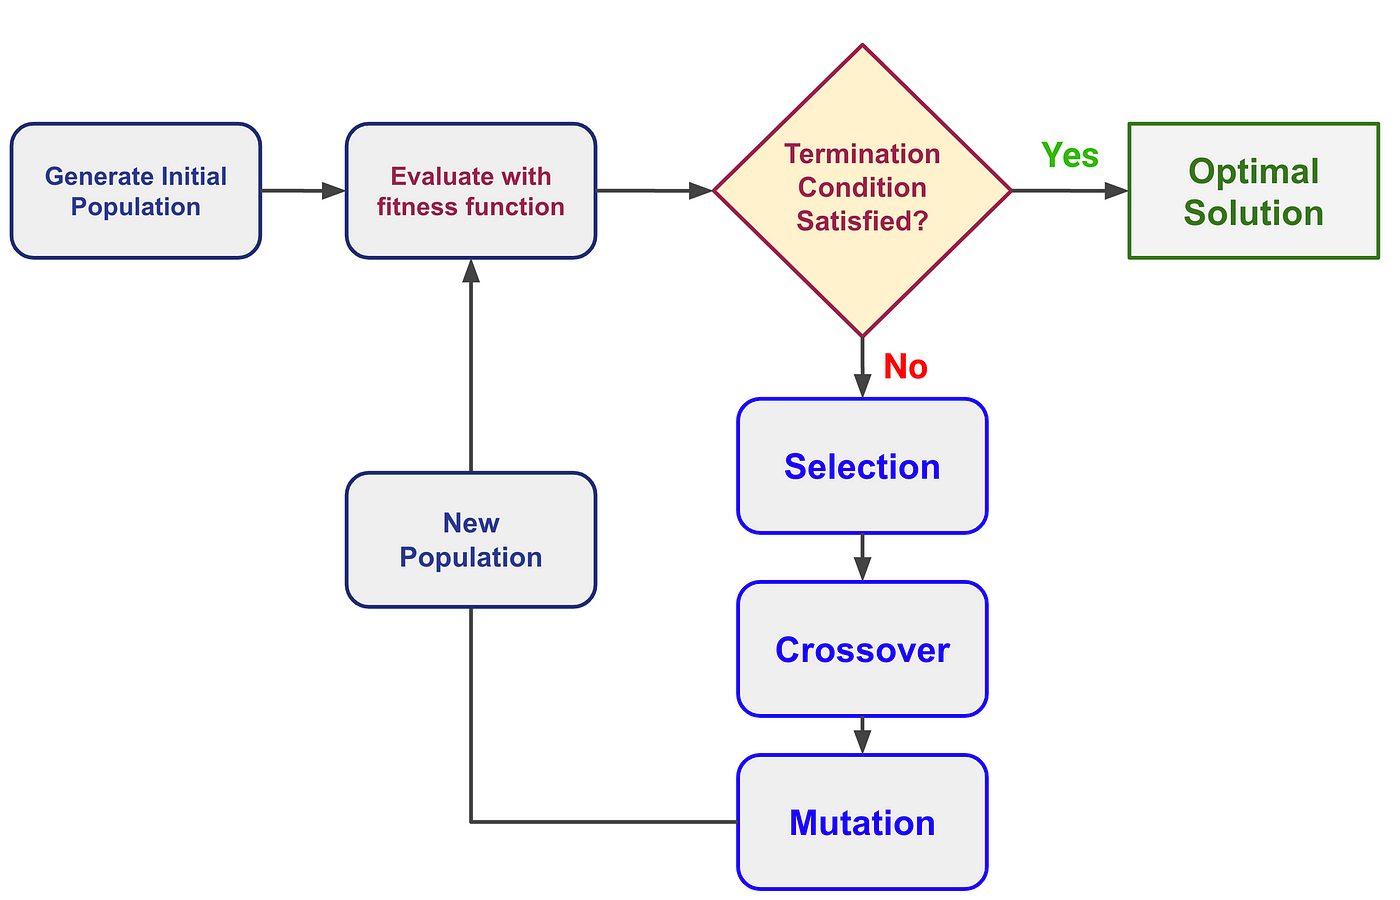
\includegraphics[
        width=\linewidth,
        height=6cm,
        keepaspectratio,
    ]{images/artificial-intelligence/searching/genetic-algorithm-flowchart.png}
    \caption{Genetic Algorithm - flowchart}
\end{figure}


\begin{enumerate}
    \item A genetic algorithm (GA) is a variant of stochastic beam search in which successor states are generated by combining \textit{two} parent states rather than by modifying a single state.
    \hfill \cite{ai/book/Artificial-Intelligence-A-Modern-Approach/Russell-Norvig}

    \item Like beam searches, GAs begin with a set of k randomly generated states, called the population. 
    Each state, or individual, is represented as a string over a finite alphabet—most commonly, a string of $0$s and $1$s.
    \hfill \cite{ai/book/Artificial-Intelligence-A-Modern-Approach/Russell-Norvig}

    \item \textbf{culling}: all individuals below a given threshold are discarded, can be shown to converge faster than the random version
    \hfill \cite{ai/book/Artificial-Intelligence-A-Modern-Approach/Russell-Norvig}

    \item \textbf{steps}:
    \begin{enumerate}
        \item population states
        \hfill \cite{ai/book/Artificial-Intelligence-A-Modern-Approach/Russell-Norvig}

        \item each state is rated by the objective function, or (in GA terminology) the \textbf{fitness function}.
        A fitness function should return higher values for better states
        \hfill \cite{ai/book/Artificial-Intelligence-A-Modern-Approach/Russell-Norvig}

        \item two pairs are selected at \textbf{random} for \textbf{reproduction}, in accordance with the probabilities in (b).
        For each pair to be mated, a \textbf{crossover point} is chosen randomly from the positions in the string.
        \hfill \cite{ai/book/Artificial-Intelligence-A-Modern-Approach/Russell-Norvig}

        \item the offspring themselves are created by crossing over the parent strings at the crossover point.
        When two parent states are quite different, the crossover operation can produce a state that is a long way from either parent state. 
        It is often the case that the population is quite diverse early on in the process, so crossover (like simulated annealing) frequently takes large steps in the state space early in the search process and smaller steps later on when most individuals are quite similar
        \hfill \cite{ai/book/Artificial-Intelligence-A-Modern-Approach/Russell-Norvig}

        \item each location (gene) is subject to random \textbf{mutation} with a small independent probability. 
        \hfill \cite{ai/book/Artificial-Intelligence-A-Modern-Approach/Russell-Norvig}
    \end{enumerate}

    \item Like stochastic beam search, genetic algorithms combine an uphill tendency with random exploration and exchange of information among parallel search threads.
    \hfill \cite{ai/book/Artificial-Intelligence-A-Modern-Approach/Russell-Norvig}

    \item The primary advantage, if any, of genetic algorithms comes from the crossover operation. 
    Yet it can be shown mathematically that, if the positions of the genetic code are permuted initially in a random order, crossover conveys no advantage. 
    \hfill \cite{ai/book/Artificial-Intelligence-A-Modern-Approach/Russell-Norvig}
\end{enumerate}































\clearpage
\section{Summary}


\begin{customArrayStretch}{1.7}
\begin{longtable}{| 
>{\RaggedRight\arraybackslash}p{5cm} | 
>{\RaggedRight\arraybackslash}p{1.5cm} | 
>{\RaggedRight\arraybackslash}p{3cm} | 
>{\centering\arraybackslash}p{1cm} | 
>{\centering\arraybackslash}p{1cm} | 
>{\centering\arraybackslash}p{1cm} | 
>{\centering\arraybackslash}p{0.7cm} |}

\hline
\multirow{2}{*}{\textbf{Algorithm}} & 
\multirow{2}{*}{\textbf{Complete?}} &
\multirow{2}{*}{\textbf{Optimal?}} & 
\multicolumn{2}{c|}{\textbf{Time Complexity}} &
\multicolumn{2}{c|}{\textbf{Space Complexity}}
\\ \cline{4-7}
&&& 
\textbf{Graph} & \textbf{Tree} & 
\textbf{Graph} & \textbf{Tree}
\\ \hline
\endfirsthead

\hline
\multirow{2}{*}{\textbf{Algorithm}} & 
\multirow{2}{*}{\textbf{Complete?}} &
\multirow{2}{*}{\textbf{Optimal?}} & 
\multicolumn{2}{c|}{\textbf{Time Complexity}} &
\multicolumn{2}{c|}{\textbf{Space Complexity}}
\\ \cline{4-7}
&&& 
\textbf{Graph} & \textbf{Tree} & 
\textbf{Graph} & \textbf{Tree}
\\ \hline
\endhead

\hline\endfoot
\hline\endlastfoot


%%%%%%%%%%%%%%%%%%%%%%%%%%%%%%%%%%%%%%%%%%%%%%%%

\multicolumn{7}{|c|}{\fontsize{17}{17}\selectfont \textsc{Uninformed Search/ Blind Search}} \\ \hline

%%%%%%%%%%%%%%%%%%%%%%%%%%%%%%%%%%%%%%%%%%%%%%%%

\hyperref[AI: Algorithms/Breadth-first search (BFS)]{\textbf{Breadth-first search (BFS)}} &
YES$^3$ &
YES$^{1|2}$ &
\multicolumn{2}{c|}{$\mathcal{O}(b^d)$} &
\multicolumn{2}{c|}{$\mathcal{O}(b^d)$}
\\ \hline


\hyperref[AI: Algorithms/Uniform-cost search (UCS)]{\textbf{Uniform-cost search (UCS)}} &
YES$^4$ &
YES &
\multicolumn{2}{c|}{$\mathcal{O}(b^{1+\dfloor{C^\ast/\varepsilon}})$} &
\multicolumn{2}{c|}{$\mathcal{O}(b^{1+\dfloor{C^\ast/\varepsilon}})$}
\\ \hline


\hyperref[AI: Algorithms/Depth-first search (DFS)]{\textbf{Depth-first search (DFS)}} &
YES$^{3\&5}$ &
NO &
$\mathcal{O}(b^d)$ & $\mathcal{O}(b^m)$ &
$\mathcal{O}(bd)$ & $\mathcal{O}(bm)$
\\ \hline


\hyperref[AI: Algorithms/Backtracking Search]{\textbf{Backtracking Search}} &
YES$^{3\&5}$ &
NO &
$\mathcal{O}(b^d)$ & $\mathcal{O}(b^m)$ &
$\mathcal{O}(d)$ & $\mathcal{O}(m)$
\\ \hline


\hyperref[AI: Algorithms/Depth-limited search (DLS)]{\textbf{Depth-limited search (DLS)}} &
NO$^{6}$ &
YES$^{6}$ &
\multicolumn{2}{c|}{$\mathcal{O}(b^\ell)$} &
\multicolumn{2}{c|}{$\mathcal{O}(b\ell)$}
\\ \hline


\hyperref[AI: Algorithms/Iterative Deepening Search (IDS)]{\textbf{Iterative Deepening Search (IDS)}} &
YES$^{3}$ &
YES$^{1|2}$ &
\multicolumn{2}{c|}{$\mathcal{O}(b^d)$} &
\multicolumn{2}{c|}{$\mathcal{O}(bd)$}
\\ \hline


\hyperref[AI: Algorithms/Iterative Lengthening Search (ILS)]{\textbf{Iterative Lengthening Search (ILS)}} &
YES$^{4}$ &
YES &
\multicolumn{2}{c|}{$\mathcal{O}(b^{1+\dfloor{C^\ast/\varepsilon}})$} &
\multicolumn{2}{c|}{$\mathcal{O}(bC^\ast/\varepsilon)$}
\\ \hline


\hyperref[AI: Algorithms/Bidirectional search]{\textbf{Bidirectional search}} &
YES$^{7}$ &
YES$^{2\&8}$ &
\multicolumn{2}{c|}{$\mathcal{O}(b^{d/2})$} &
\multicolumn{2}{c|}{$\mathcal{O}(b^{d/2})$}
\\ \hline


%%%%%%%%%%%%%%%%%%%%%%%%%%%%%%%%%%%%%%%%%%%%%%%%

\multicolumn{7}{|c|}{\fontsize{17}{17}\selectfont \textsc{Informed Search/ Heuristic Search}} 
\\ \hline

%%%%%%%%%%%%%%%%%%%%%%%%%%%%%%%%%%%%%%%%%%%%%%%%


\hyperref[AI: Algorithms/Greedy best-first search (GBFS)]{\textbf{Greedy best-first search (GBFS)}} &
YES$^{3\&5}$ &
NO &
\multicolumn{2}{c|}{$\mathcal{O}(b^m)$} &
\multicolumn{2}{c|}{$\mathcal{O}(b^m)$}
\\ \hline


\hyperref[AI: Algorithms/A* Search]{\textbf{A* Search}} &
YES$^{3\&4}$ &
YES$^{(9\&10)|(5\&11)}$ &
\multicolumn{2}{c|}{$\mathcal{O}(
    b^\Delta)^{12}$ or 
    $\mathcal{O}(b^{\Delta_rd})^{2}$
} &
\multicolumn{2}{c|}{$\mathcal{O}()$}
\\ \hline













\end{longtable}
\end{customArrayStretch}

\vspace{0.5cm}
\textbf{Conditions}:
\vspace{0.2cm}
\begin{enumerate}[itemsep=0.1cm]
% 1
\item path cost is a non-decreasing function of the depth of the node
% 2
\item step costs are all identical
% 3
\item branching factor $b$ is finite (number of states are finite)
% 4
\item every step exceeds some small positive constant $\varepsilon > 0$
% 5
\item graph version is used
% 6
\item $\ell < d$
% 7
\item additional search is used to make sure the path isn’t another short-cut across the gap
% 8
\item both directions use breadth-first search
% 9
\item tree version is used
% 10
\item $h(n)$ is admissible
% 11
\item $h(n)$ is consistent
% 12
\item in the maximum absolute error
\end{enumerate}


\vspace{0.5cm}
\textbf{Notation Interpretation}:
\vspace{0.2cm}
\begin{enumerate}[itemsep=0.2cm]

\item YES$^{a|b}$ = YES \textbf{if} either $a$ \textbf{or} $b$ must satisfy \textbf{else} NO

\item YES$^{a\&b}$ = YES \textbf{if} either $a$ \textbf{and} $b$ must satisfy \textbf{else} NO

\end{enumerate}
















